\documentclass[border=10pt]{standalone}
\usepackage{tikz}
\usetikzlibrary{shapes}
\tikzset{utriangle/.style = {regular polygon, regular polygon sides=3, inner sep=0.5pt}}
\tikzset{btriangle/.style = {regular polygon, regular polygon sides=3, shape border rotate=180,
        inner sep=0.5pt}}

\begin{document}
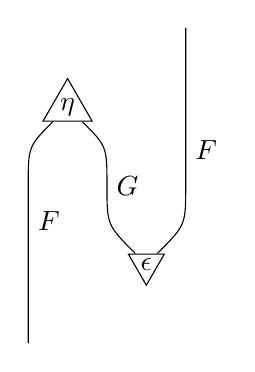
\begin{tikzpicture}[baseline=(current bounding box.center),]
\path coordinate[] (tikzsd_internal_pos_0_0) at (2.0,0.0);
\path coordinate[] (tikzsd_internal_pos_1_0) at (0.0,-2.0);
\path coordinate[] (tikzsd_internal_pos_1_1) at (1.0,-2.0);
\path coordinate[] (tikzsd_internal_pos_1_2) at (2.0,-2.0);
\path coordinate[] (tikzsd_internal_pos_2_0) at (0.0,-4.0);

\path node[utriangle,draw,] (tikzsd_internal_nt_node_0_0) at (0.5,-1.0) {$\eta$};
\path node[btriangle,draw,] (tikzsd_internal_nt_node_1_0) at (1.5,-3.0) {$\epsilon$};

\path [draw] (tikzsd_internal_nt_node_0_0) ..controls(0.0,-1.5)..(tikzsd_internal_pos_1_0) ..controls(0.0,-2.5)and(0.0,-3.5)..(tikzsd_internal_pos_2_0) node[pos=0.25,auto,] {$F$};
\path [draw] (tikzsd_internal_nt_node_0_0) ..controls(1.0,-1.5)..(tikzsd_internal_pos_1_1) ..controls(1.0,-2.5)..(tikzsd_internal_nt_node_1_0) node[pos=0.0,auto,] {$G$};
\path [draw] (tikzsd_internal_pos_0_0) ..controls(2.0,-0.5)and(2.0,-1.5)..(tikzsd_internal_pos_1_2) node[pos=0.75,auto,] {$F$} ..controls(2.0,-2.5)..(tikzsd_internal_nt_node_1_0);
\end{tikzpicture}
\end{document}
